% ---------------------------------------------------------------------------
% Author guideline and sample document for EG publication using LaTeX2e input
% D.Fellner, v1.13, Jul 31, 2008

\documentclass{egpubl}
\usepackage{eurovis2019}

% --- for  Annual CONFERENCE
% \ConferenceSubmission   % uncomment for Conference submission
% \ConferencePaper        % uncomment for (final) Conference Paper
% \STAR                   % uncomment for STAR contribution
% \Tutorial               % uncomment for Tutorial contribution
% \ShortPresentation      % uncomment for (final) Short Conference Presentation
% \Areas                  % uncomment for Areas contribution
% \MedicalPrize           % uncomment for Medical Prize contribution
% \Education              % uncomment for Education contribution
% \Poster                 % uncomment for Poster contribution
% \DC                     % uncomment for Doctoral Consortium
%
% --- for  CGF Journal
% \JournalSubmission    % uncomment for submission to Computer Graphics Forum
% \JournalPaper         % uncomment for final version of Journal Paper
%
% --- for  CGF Journal: special issue
% \SpecialIssueSubmission    % uncomment for submission to , special issue
% \SpecialIssuePaper         % uncomment for final version of Computer Graphics Forum, special issue
%                          % EuroVis, SGP, Rendering, PG
% --- for  EG Workshop Proceedings
% \WsSubmission      % uncomment for submission to EG Workshop
% \WsPaper           % uncomment for final version of EG Workshop contribution
% \WsSubmissionJoint % for joint events, for example ICAT-EGVE
% \WsPaperJoint      % for joint events, for example ICAT-EGVE
% \Expressive        % for SBIM, CAe, NPAR
% \DigitalHeritagePaper
% \PaperL2P          % for events EG only asks for License to Publish

% --- for EuroVis 
% for full papers use \SpecialIssuePaper
% \STAREurovis   % for EuroVis additional material 
\EuroVisPoster % for EuroVis additional material 
% \EuroVisShort  % for EuroVis additional material

 \electronicVersion % can be used both for the printed and electronic version

% !! *please* don't change anything above
% !! unless you REALLY know what you are doing
% ------------------------------------------------------------------------

% for including postscript figures
% mind: package option 'draft' will replace PS figure by a filename within a frame
\ifpdf \usepackage[pdftex]{graphicx} \pdfcompresslevel=9
\else \usepackage[dvips]{graphicx} \fi

\PrintedOrElectronic

% prepare for electronic version of your document
\usepackage{t1enc,dfadobe}

\usepackage{egweblnk}
\usepackage{cite}

% For backwards compatibility to old LaTeX type font selection.
% Uncomment if your document adheres to LaTeX2e recommendations.
% \let\rm=\rmfamily    \let\sf=\sffamily    \let\tt=\ttfamily
% \let\it=\itshape     \let\sl=\slshape     \let\sc=\scshape
% \let\bf=\bfseries

% end of prologue
% ---------------------------------------------------------------------
% EG author guidelines plus sample file for EG publication using LaTeX2e input
% D.Fellner, v2.02, Jan 25, 2017


\title[Improving the Scalability of Interactive Visualization Systems for Exploring Threaded Conversations]%
      {Improving the Scalability of Interactive Visualization Systems for Exploring Threaded Conversations}

% for anonymous conference submission please enter your SUBMISSION ID
% instead of the author's name (and leave the affiliation blank) !!
% for final version: please provide your *own* ORCID in the brackets following \orcid; see https://orcid.org/ for more details.
\author[A. McNutt \& G. Kindlmann]
{\parbox{\textwidth}{\centering A. McNutt, IEEE student member, \& G. Kindlmann
%        S. Spencer$^2$\thanks{Chairman Siggraph Publications Board}  
        }
        \\
% For Computer Graphics Forum: Please use the abbreviation of your first name.
{\parbox{\textwidth}{\centering Department of Computer Science, University of Chicago
%        $^2$ Another Department to illustrate the use in papers from authors
%             with different affiliations
       } 
}
}
% ------------------------------------------------------------------------

% if the Editors-in-Chief have given you the data, you may uncomment
% the following five lines and insert it here
%
% \volume{36}   % the volume in which the issue will be published;
% \issue{1}     % the issue number of the publication
% \pStartPage{1}      % set starting page


%-------------------------------------------------------------------------
\begin{document}

\teaser{
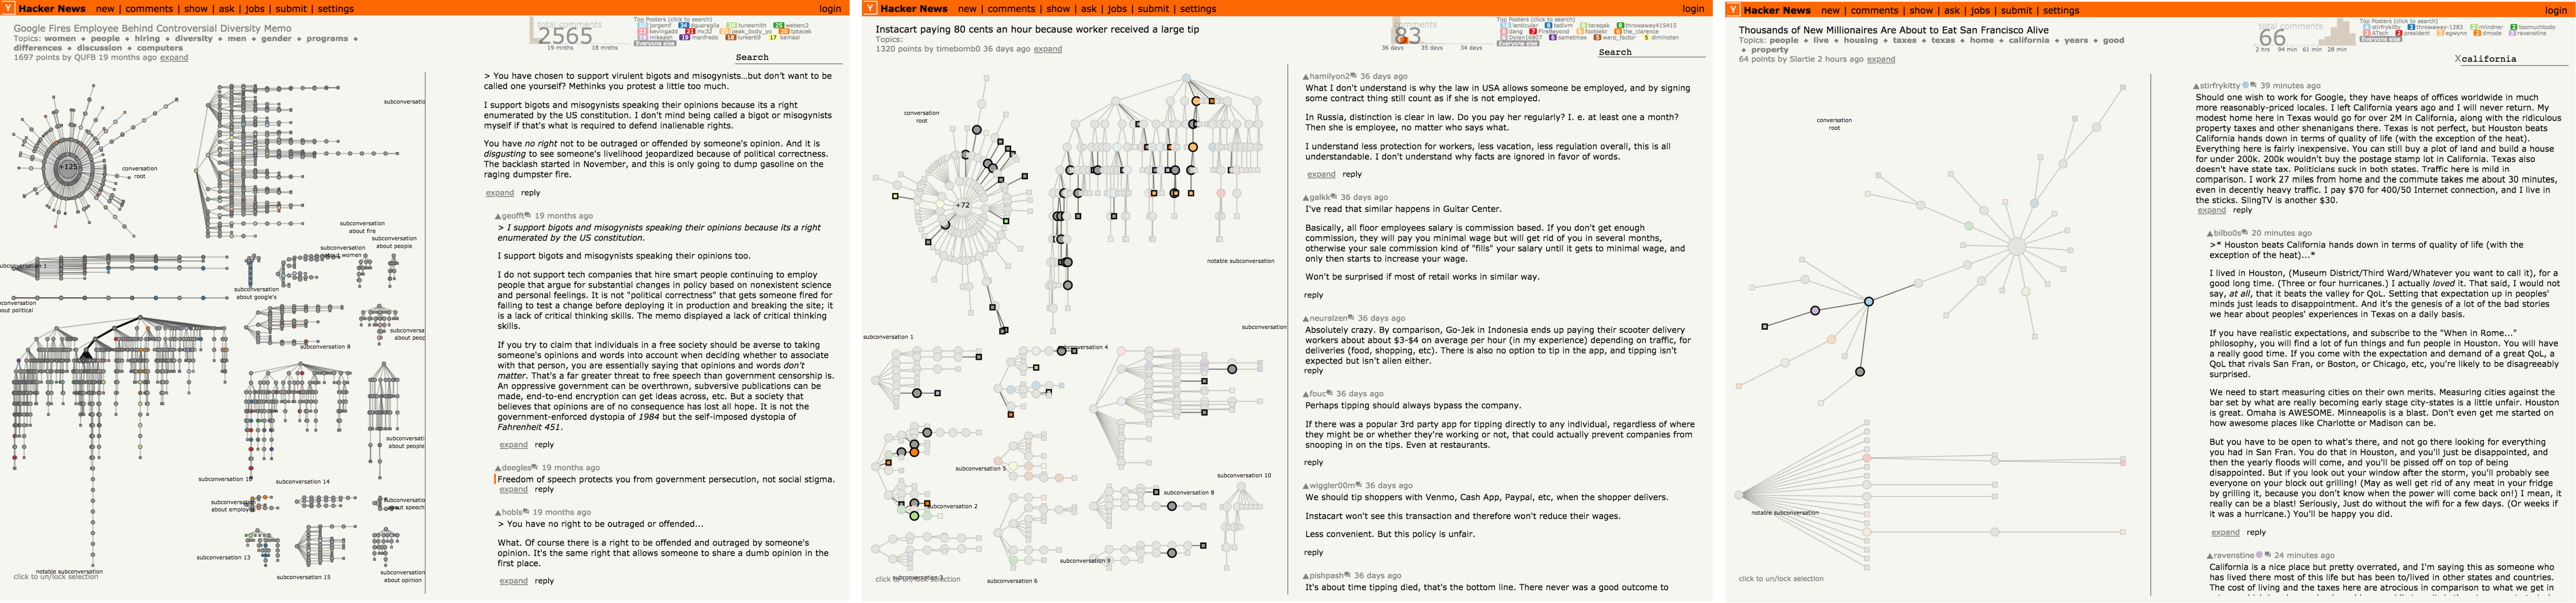
\includegraphics[width=\linewidth]{images/teaser.pdf}
\centering
\caption{
Two very differently sized HackerNews conversations (715 and 85 comments respectively) rendered using our ForumExplorer application.
%
The right image shows a temporal search state.
}
\label{fig:teaser}
}

\maketitle
%-------------------------------------------------------------------------
\begin{abstract}
   The ABSTRACT is to be in fully-justified italicized text, 
   between two horizontal lines,
   in one-column format, 
   below the author and affiliation information. 
   Use the word ``Abstract'' as the title, in 9-point Times, boldface type, 
   left-aligned to the text, initially capitalized. 
   The abstract is to be in 9-point, single-spaced type.
   The abstract may be up to 3 inches (7.62 cm) long. \\
   Leave one blank line after the abstract, 
   then add the subject categories according to the ACM Classification Index 
%-------------------------------------------------------------------------
%  ACM CCS 1998
%  (see http://www.acm.org/about/class/1998)
% \begin{classification} % according to http:http://www.acm.org/about/class/1998
% \CCScat{Computer Graphics}{I.3.3}{Picture/Image Generation}{Line and curve generation}
% \end{classification}
%-------------------------------------------------------------------------
%  ACM CCS 2012
   (see http://www.acm.org/about/class/class/2012)
%The tool at \url{http://dl.acm.org/ccs.cfm} can be used to generate
% CCS codes.
%Example:
\begin{CCSXML}
<ccs2012>
<concept>
<concept_id>10010147.10010371.10010352.10010381</concept_id>
<concept_desc>Computing methodologies~Collision detection</concept_desc>
<concept_significance>300</concept_significance>
</concept>
<concept>
<concept_id>10010583.10010588.10010559</concept_id>
<concept_desc>Hardware~Sensors and actuators</concept_desc>
<concept_significance>300</concept_significance>
</concept>
<concept>
<concept_id>10010583.10010584.10010587</concept_id>
<concept_desc>Hardware~PCB design and layout</concept_desc>
<concept_significance>100</concept_significance>
</concept>
</ccs2012>
\end{CCSXML}

\ccsdesc[300]{Computing methodologies~Collision detection}
\ccsdesc[300]{Hardware~Sensors and actuators}
\ccsdesc[100]{Hardware~PCB design and layout}


\printccsdesc   
\end{abstract}





%-------------------------------------------------------------------------
\section{Introduction}


%%%
%%% Figure 1
%%%
\begin{figure}[htb]
\centering
% the following command controls the width of the embedded PS file
% (relative to the width of the current column)
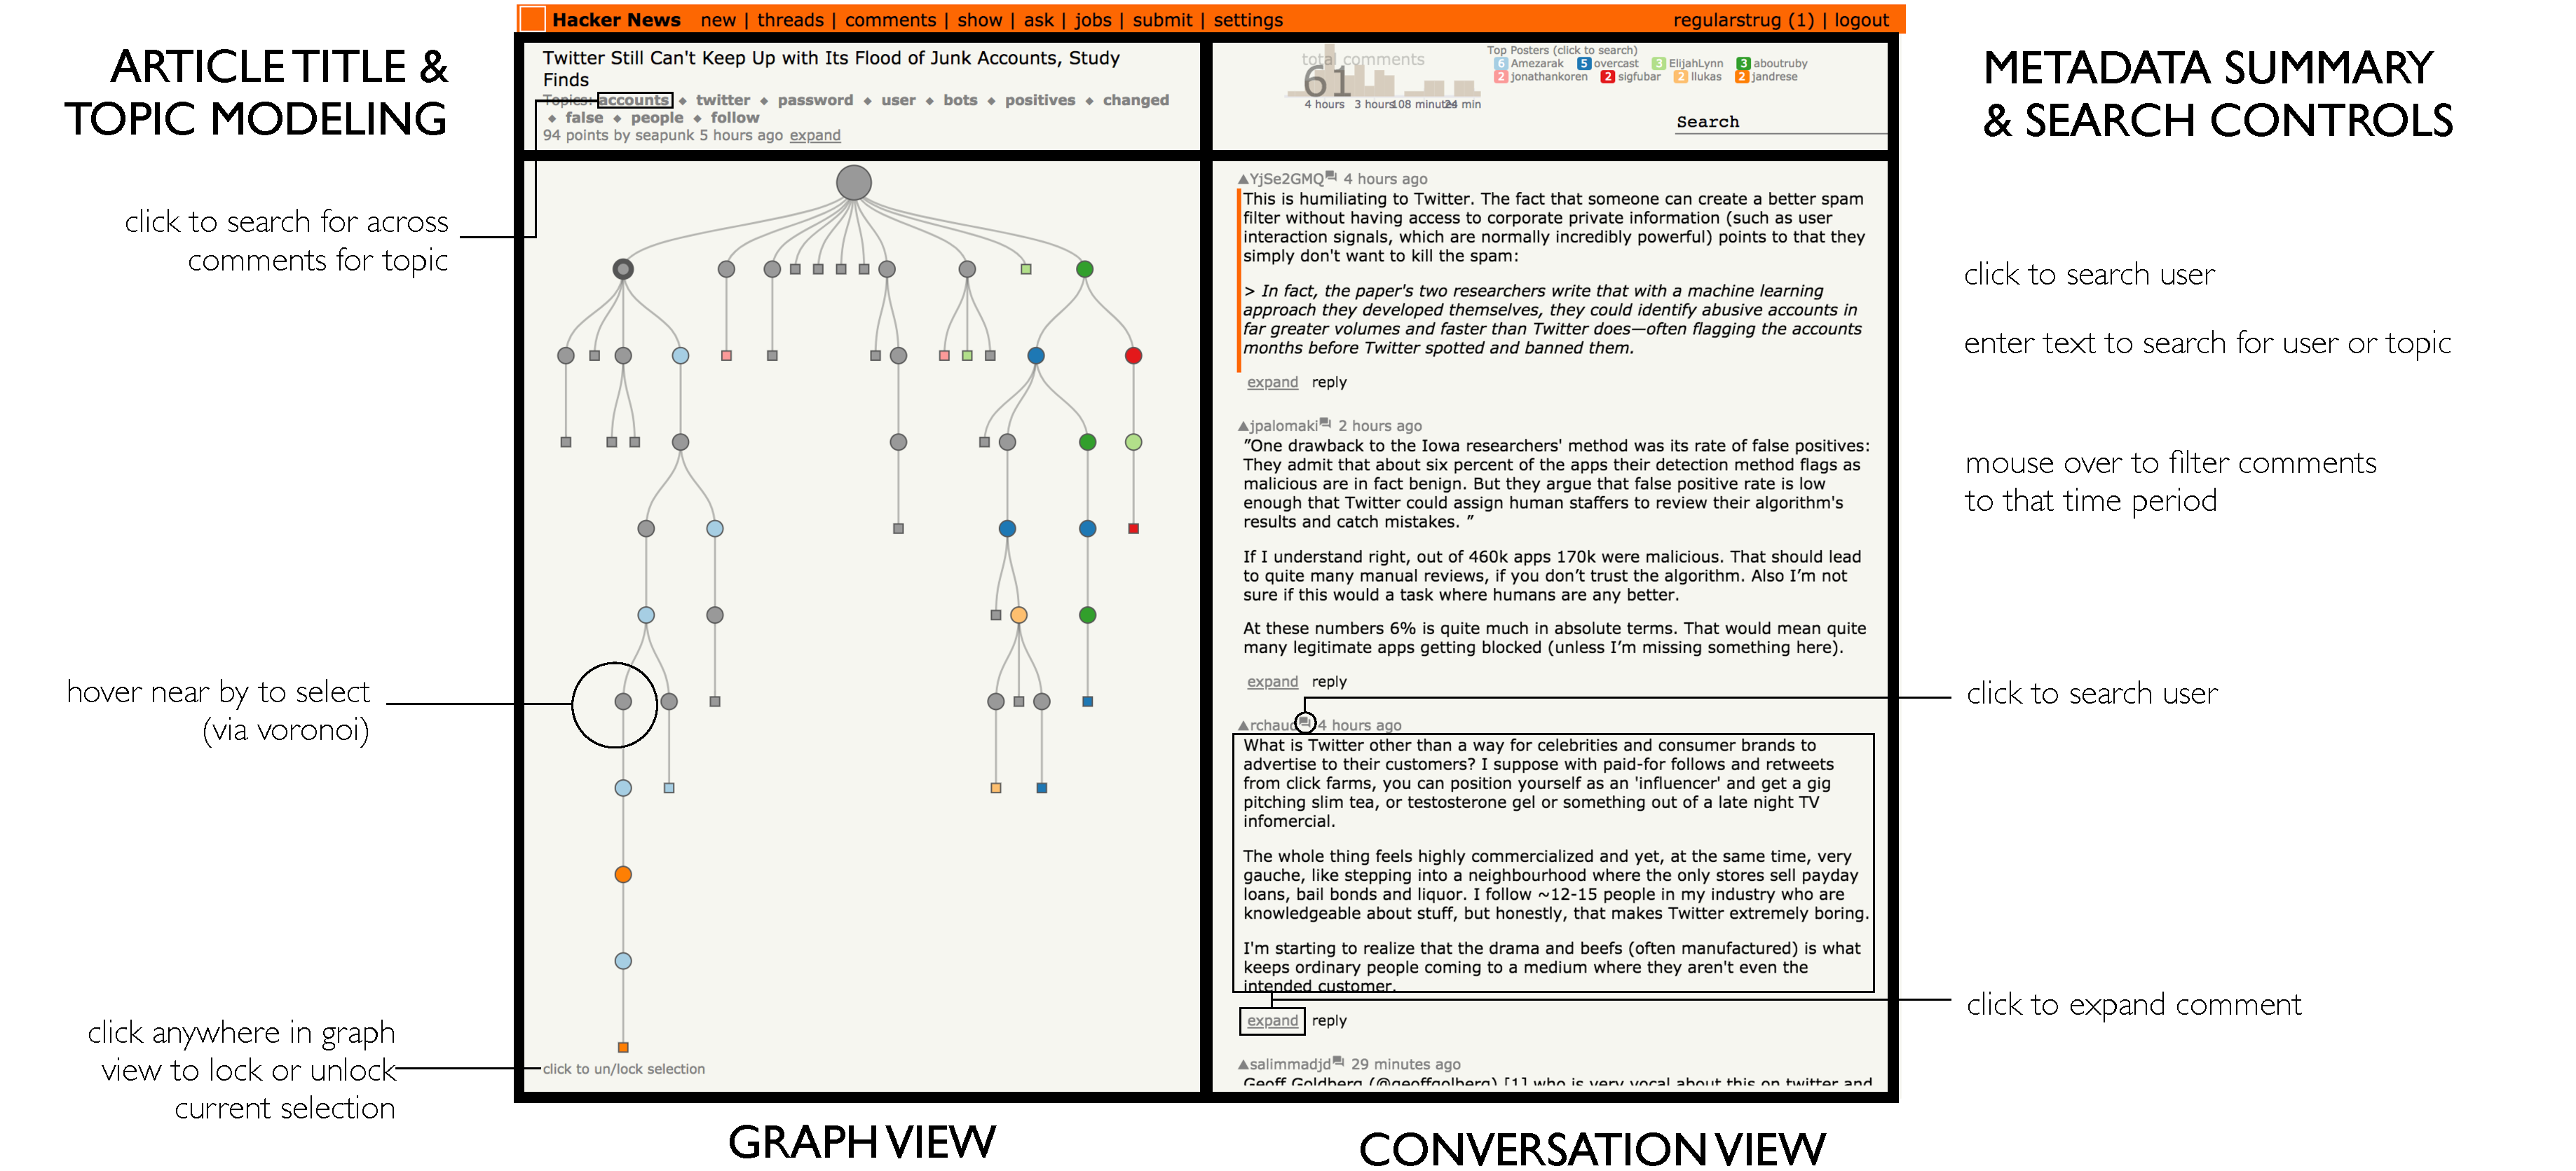
\includegraphics[width=\linewidth]{images/explainer.pdf}
% replacing the above command with the one below will explicitly set
% the bounding box of the PS figure to the rectangle (xl,yl),(xh,yh).
% It will also prevent LaTeX from reading the PS file to determine
% the bounding box (i.e., it will speed up the compilation process)
% \includegraphics[width=.95\linewidth, bb=39 696 126 756]{sampleFig}
%
%  \parbox[t]{.9\columnwidth}{\relax
%          For all figures please keep in mind that you \textbf{must not}
%         use images with transparent background! 
%         }
%
\caption{
\label{fig:explainer}
Annotated view explaining the components of the UI.
}
\end{figure}


Conversation on the internet takes many forms and shapes, including question+answer forums, synchronous messaging, and asynchronous threaded conversation. Of particular interest are conversations that take place in an asynchronous threaded environments, such as reddit or slash dot, as they offer a mechanism for communities to have wide collections of related conversations within a single topic. In many cases the participants in these conversations are experts on the topic and might provide valuable insights. Unfortunately the design of these digital spaces typically do not allow for users to interact with the conversational corpus as a whole, which can limit or impede understanding of the community opinions and insights about a topic.

Building systems that provide an overview of a complex or non-linear data space is a favorite class of problems in the information visualization community, and threaded conversations have been no exception. Previous visualization works have developed a fascinating collection of UI paradigms to address this space. A common trend among these works features a overview of the conversational thread by representing it as graph like structure, which the user then interacts with in a details-on-demand \cite{shneiderman1996eyes} pattern to expose components of the discourse. While these tools are uniformly well received by their evaluation audiences, they have failed to gain widespread usage; possibly because they do not possess an accessible or online implementations, are not aligned to the specific community they are trying to affect, and are designed around a single ideal size of conversation (and thus become cumbersome or difficult to use when conversations of interest fall outside of that target domain). Further, it is possible that this type of tool is in fact not necessary for the types of tasks that most users pursue within these spaces.

In this work we present Forum Explorer, a Chrome Extension that repurposes the conventional layout of yCombinator's HackerNews \cite{hackernews} to facilitate better data exploration through the use of tree visualization techniques. Our system expands upon previous techniques developed and contributes several novel visual encodings to facilitate. Specifically, we introduce a novel Forested Tree View which splits threaded conversations at the root into a collection of smaller and more legible trees, this allows for ample visual space to provide in-situ annotations and textual guides. We construct a solution for reducing visual noise in large conversations by collapsing rooted stumps into the root, while still making those nodes available. Our solution seeks to make this type of tool easily available through the use of easily reproducible components.

 
 \section{Related Work}
 
 Previous work on this topic has developed a number of different strategies for displaying and facilitating novel user interactions under a variety of different design goals. The first work of this type appears to be Donath et al's Loom, which introduced the graphical exploration of comments as a collection of nodes in space connected together through polylines \cite{donath1999visualizing}. This was quickly followed by Sack's Conversation Map which added a more tree-like structure to the display \cite{sack2000conversation}. Watternberg et al present a pair of papers which appear to be the first instance of a split pane view, with one providing the graphical overview (which was a graphical abstraction of the multiply indented form threaded conversation are usually depicted in) and the other displaying comments \cite{wattenberg2003conversation, dave2004flash}. Pascual-Cid et al introduce a space filling radial tree layout.  Narayan construct tldr which focuses on reddit and encodes the tree as an icicle diagram \cite{narayan2010not}.  Hoque et al's family of tools breaks from purely metadata visualization by adding NLP-based-summaries like faceted topic modeling and sentiment analysis on top of a split pane interaction with a abstracted indentation graphical summary\cite{hoque2014convis, hoque2016interactive}. These tools provide valuable insight, but come at the cost of forcing their users to use an unfamiliar environment, as well as being not being actually deployed. Most closely related to our technical approach is Treeverse, a chrome extension which allows users to visualize the conversation graph associated with a particular tweet.\cite{treeverse}  When the user is engaged with a particular tweet they can opt into the Treeverse view which renders the graph as a click and draggable tree with associated secondary panel. Our work improves over this design in that it tightens the response interaction response cycle and enables the user to extract useful information from a single view.

Each of these works features a ringingly positive user evaluation. It is unclear whether or not this result is due to the novelty of the system, and therein experiment bias, or the true utility of the tool. The best evidence that this type of system has substantive utility is that it used by Rao et al \cite{twittercanoes} to study the way that twitter is used SOMTHING domain specific knowledge sharing discussions. This suggests this type of data exploration tool has utility beyond academia.


\section{Forum Explorer}

TODO NEED TO SCRAPE HACKERNEWS TO FIGURE OUT MAX COMMENT THREAD

We implement a split pane view in which a graphical overview is presented on the left and a detail view on the right. The graphical overview consists of a one of a collection of tree visualizations with the origin comment represents as the root of the tree.

We provide additional detail about the UI in Figure \ref{fig:explainer}. In addition to our Forested View we provide several additional view options to enable users a sense of play and to facilitate exploration within the tool, these include an unsegmented radial layout, a reinfold-something tidy tree CITATION, a gridded tree CITATION, and an orbit layout CITATION. 


Our primary contribution in this work is addition of a novel visual encoding in the overview representation. We observe that many presentation of trees such as THE RADIAL TREE ONE OR CONVIS scale poorly when presented a large collection of nodes. To address this issue we observe that their tends to be zipfs law distribution of weights for branches incident to the root, so we prune the heaviest branches and layout them out as adjacent conversations 


%-------------------------------------------------------------------------
\section{Conclusions \& Future Work}

We have presented Forum Explorer, a tool for exploring threaded conversations on HackerNews. Our primary contribution is a novel Forested Tree layout that facilitates better scalability for systems of this type.


The specific utility of this type of conversation overview tool remains unclear, although based contemporary developments, such as Treeverse's 2412 active installs as well as it's usage in 

Previous studies of threaded conversation have typically involved a small scale user study, SPECIFICS. While these studies usefully demonstrate the usability of the structural design elements in general, their context as laboratory based analyses precludes them from providing longitudinal information about the way users might interact with this type of tool when they are able to incorporate it into their day to day workflow. Forum Explorer is well positioned 

Our current design process has, in the lens of data feminism, been unfeminist. Our design process happened without consultation of those who might find the application (other than perhaps ourselves). While we are able to rest on the many of the observations from ConVis's prior user studies in the topic, individual forum users tend to have individual expectations about their tools.

The specific utility of this type of conversation overview tool remains unclear, the lessons learned from ours and other systems could readily be applied to graph analysis problems of a similar size and scale. Analysis of locally relevant articles in the scholarship graph are one such example of this type of system.




%-------------------------------------------------------------------------

%\bibliographystyle{eg-alpha}
\bibliographystyle{eg-alpha-doi}

\bibliography{forum-bib}

\end{document}

